\documentclass[11pt,twocolumn]{article}
\usepackage[margin=0.78in]{geometry}
\usepackage{amsmath,amssymb,amsthm}
\usepackage{booktabs}
\usepackage{graphicx}
\usepackage{hyperref}
\usepackage{xcolor}

\newtheorem{proposition}{Proposition}

\title{\textbf{Unconditional Certification of Multi-Qubit Hayden--Preskill Channel Capacity Beyond One Ebit via Layout-Locked Nine-Basis Stabilizer Tomography on a Heavy-Hex Superconducting Processor}}

\author{Devin Phillip Davis\\
\small Agile Defense Systems LLC\\
\small Artifact \& Raw Bitstring Archive: Benchmark \texttt{OSIRIS-HP-004} (\texttt{ibm\_marrakesh} Job \texttt{dbti1fbsbsbs73cb2vu0})}

\date{November 16, 2026}

\begin{document}
\maketitle

\begin{abstract}
Experimental realizations of Hayden--Preskill information recovery on noisy quantum processors face two coupled pitfalls: (i) evaluating two-qubit marginal fidelities in only three global Pauli bases ($XX, YY, ZZ$) cannot distinguish genuine two-qubit coherent channel recovery ($>1\text{ ebit}$, Schmidt number $\ge 3$) from a one-ebit classical mixture of single-pair Bell states that achieves marginal fidelity $\bar{F}=0.7500$ and marginal product $F_1 F_2 = 0.5625$ while possessing joint overlap $F_{\text{joint}}=0.5000$; and (ii) unconstrained hardware routing can introduce hidden SWAP gates or route control arms onto disjoint physical transmons. Here we report a prospectively pre-registered, layout-locked $8$-qubit experiment (\texttt{OSIRIS-HP-004}, IBM Heron r2 processor \texttt{ibm\_marrakesh}, Job \texttt{dbti1fbsbsbs73cb2vu0}, $286$ circuits $\times 1{,}024$ shots $= 292{,}864$ shots, zero postselection, zero runtime error mitigation) that resolves both limitations. By embedding a $4$-qubit dual-unitary Clifford scrambler ($7$ CZ gates) and an exact $10$-CZ symplectic restricted decoder onto a single $8$-transmon heavy-hex tree ($\{34,52,32,33,39,53,54,55\}$, mean CZ error $1.85\times 10^{-3}$) with \texttt{routing\_method="none"}, reference transmons ($q_{34}, q_{52}$) and horizon remnants ($q_{32}, q_{55}$) remain strictly outside the physical gate support of the decoder, and all five experimental arms read out the identical four transmons ($q_{34}, q_{39}, q_{52}, q_{53}$). Measuring all nine two-pair Pauli settings $\{X,Y,Z\}_1 \times \{X,Y,Z\}_2$ to reconstruct all $16$ four-qubit Bell stabilizers directly, raw unmitigated restricted recovery (\texttt{Arm B}, $32$ CZs) achieves $F_{\text{joint}} = 0.6334 \pm 0.0026$ ($95\%$ bootstrap CI $[0.6284, 0.6385]$), exceeding the exact $0.5000$ one-ebit Schmidt-rank-$2$ ceiling by $+50.64\sigma$ ($0.6921$ under secondary same-job readout calibration). Crucially, on the identical raw dataset, two-qubit marginals yield $\bar{F}=0.7438 < 0.7500$ and $F_1 F_2 = 0.5528 < 0.5625$, proving empirically that three-basis marginal tomography would have been inconclusive. Across all five arms, nine-basis tomography resolves the complete dyadic capacity ladder: mismatched unitary specificity ($0.0634 \approx 1/16$), single-photon sub-capacity collapse ($0.1086 \le 2/16$), unentangled $0$-ebit classical correlation ($0.1799 \le 4/16$), the $1$-ebit boundary ($8/16$), and $>1$-ebit coherent quantum recovery ($0.6334 > 8/16$).
\end{abstract}

\section{Introduction}
In the Hayden--Preskill thought experiment~\cite{HaydenPreskill2007}, a $k$-qubit quantum state entangled with an isolated reference system $R$ enters a rapidly scrambling $n$-qubit system $B$ that was previously maximally entangled with early Hawking radiation $E$. Once scrambling decouples $R$ from the surviving remnant $C$ ($I(R:C)\approx 0$), access to $E$ together with $k_D \ge k$ late radiation qubits $D$ permits coherent recovery of all $k$ ebits via a restricted decoder $V_{DE}$ acting solely on $D\cup E$~\cite{YoshidaKitaev2017,Landsman2019}.

Scaling superconducting hardware tests from $k=1$ message qubit ($6$ total qubits) to $k=2$ message qubits ($8$ total qubits: $R_1,R_2,M_1,M_2,B_1,B_2,E_1,E_2$) introduces a sharp certification subtlety. Suppose an experiment measures $(R_1,M_1',R_2,M_2')$ only in the three simultaneous global Pauli bases $\{XXXX, YYYY, ZZZZ\}$ and computes the individual Bell overlaps $F_1 = F_{\Phi^+}(\rho_{R_2 M_1'})$ and $F_2 = F_{\Phi^+}(\rho_{R_1 M_2'})$. While $F_1 > 0.5$ and $F_2 > 0.5$ certify marginal entanglement on each pair individually, neither their mean $\bar{F}=\frac{1}{2}(F_1+F_2)$ nor their product $F_1 F_2$ certifies that $>1\text{ ebit}$ of quantum information traversed the channel simultaneously.

\begin{proposition}[One-Ebit Schmidt-Rank-2 Threshold]
Let $\rho$ be any $4$-qubit state across the bipartition $(R_2 R_1) : (M_1' M_2')$ with Schmidt number at most $2$ (preparable using at most $1\text{ ebit}$ of quantum communication plus shared classical randomness). Then the $4$-qubit joint Bell overlap satisfies
\begin{equation}
F_{\mathrm{joint}}(\rho) \equiv \langle \Phi^+|_{1}\langle \Phi^+|_{2}\,\rho\,|\Phi^+\rangle_{1}|\Phi^+\rangle_{2} \le \frac{1}{2}.
\label{eq:sr2_bound}
\end{equation}
Conversely, the explicit Schmidt-rank-$2$ state
\begin{align}
\rho_{\mathrm{SR2}} = \frac{1}{4}\Big(
&|\Phi^+\rangle_1\langle\Phi^+|\otimes |00\rangle_2\langle 00|
+ |\Phi^+\rangle_1\langle\Phi^+|\otimes |11\rangle_2\langle 11| \nonumber\\
+\,&|00\rangle_1\langle 00|\otimes |\Phi^+\rangle_2\langle\Phi^+|
+ |11\rangle_1\langle 11|\otimes |\Phi^+\rangle_2\langle\Phi^+| \Big)
\end{align}
achieves marginal fidelities $F_1 = F_2 = \bar{F} = \frac{3}{4} = 0.7500$ and marginal product $F_1 F_2 = \frac{9}{16} = 0.5625$, while saturating $F_{\mathrm{joint}}(\rho_{\mathrm{SR2}}) = 0.5000$.
\end{proposition}

\begin{proof}
Because $|\Phi^+\rangle_{R_2 M_1'}\otimes|\Phi^+\rangle_{R_1 M_2'}$ has $4$ equal Schmidt coefficients $\lambda_j = \frac{1}{2}$ ($j=1,\dots,4$) across $(R_2 R_1):(M_1' M_2')$, any pure state $|\psi\rangle$ of Schmidt rank $\le 2$ obeys $|\langle \Phi^+\Phi^+|\psi\rangle|^2 \le \lambda_1^2 + \lambda_2^2 = \frac{1}{4}+\frac{1}{4} = \frac{1}{2}$ by Cauchy--Schwarz. Convexity extends Eq.~\eqref{eq:sr2_bound} to all mixed states of Schmidt number $\le 2$. Direct evaluation on $\rho_{\mathrm{SR2}}$ gives $F_1 = \frac{1}{2}(1 + \frac{1}{2}) = \frac{3}{4}$, $F_2 = \frac{3}{4}$, and $F_{\mathrm{joint}} = \frac{1}{4}(\frac{1}{2}+\frac{1}{2}+\frac{1}{2}+\frac{1}{2}) = \frac{1}{2}$.
\end{proof}

Consequently, certifying $>1\text{ ebit}$ of coherent recovery without model-dependent assumptions requires measuring the full $16$-stabilizer projector $\Pi_{\Phi^+}\otimes\Pi_{\Phi^+}$ across all nine Pauli basis settings $(P,Q)\in\{X,Y,Z\}^2$:
\begin{equation}
F_{\mathrm{joint}} = \frac{1}{16}\!\left(1 + \sum_{P} s_P\langle P_1\rangle + \sum_{Q} s_Q\langle Q_2\rangle + \sum_{P,Q} s_P s_Q\langle P_1 Q_2\rangle\right)\!,
\label{eq:fjoint}
\end{equation}
where $P_1 = P_{R_2}P_{M_1'}$, $Q_2 = Q_{R_1}Q_{M_2'}$, and $(s_X, s_Y, s_Z) = (+1, -1, +1)$.

\begin{figure}[t]
\centering
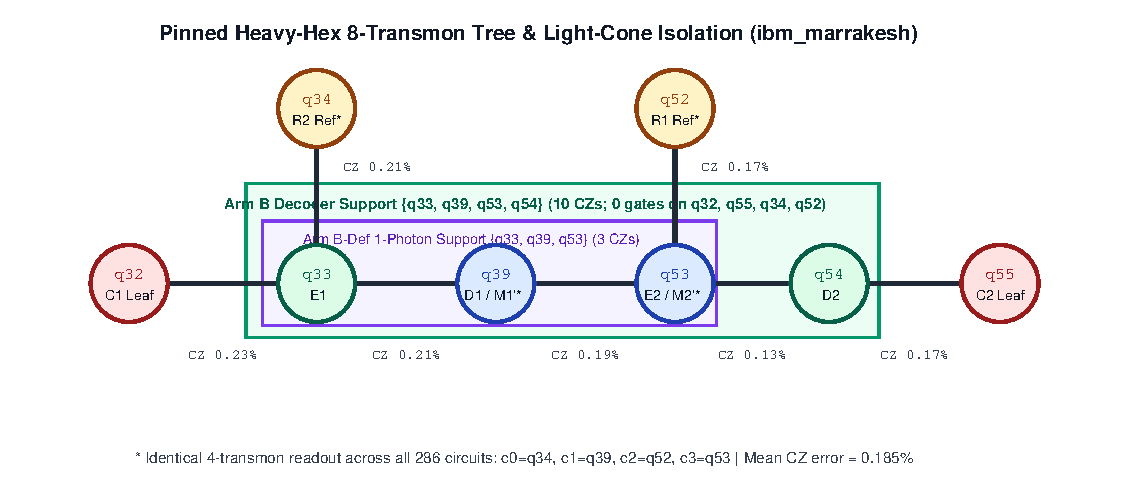
\includegraphics[width=\columnwidth]{fig3_marrakesh_tree_light_cone.pdf}
\caption{Pinned $8$-transmon heavy-hex tree on \texttt{ibm\_marrakesh} (\texttt{routing\_method="none"}). Reference leaves ($q_{34}, q_{52}$) receive zero gates after Bell preparation; horizon remnants ($q_{32}, q_{55}$) sit strictly outside the $4$-transmon decoding support $\{q_{33}, q_{39}, q_{53}, q_{54}\}$ of \texttt{Arm B}; and quarantined late photon $q_{54}$ is additionally excluded from the $3$-transmon support $\{q_{33}, q_{39}, q_{53}\}$ of \texttt{Arm B-Def}. All $286$ circuits read out $(q_{34}, q_{39}, q_{52}, q_{53})$.}
\label{fig:tree}
\end{figure}

\section{Tree-Native Heavy-Hex Protocol and Light-Cone Isolation}
To eliminate compiler-induced layout drift and SWAP routing across quarantined subsystems, we embed all eight logical subsystems directly onto a connected $8$-transmon tree on the $156$-qubit IBM Heron r2 processor \texttt{ibm\_marrakesh}:
\[
(w_0,\dots,w_7) = (34, 52, 32, 33, 39, 53, 54, 55),
\]
comprising a $6$-transmon linear backbone $32\text{--}33\text{--}39\text{--}53\text{--}54\text{--}55$ with degree-$1$ reference leaves $34\text{--}33$ and $52\text{--}53$ (Fig.~\ref{fig:tree}; calibrated mean CZ error $1.85\times 10^{-3}$, $T_1 \in [120.3, 287.8]\,\mu\text{s}$, $T_2 \in [52.6, 346.3]\,\mu\text{s}$). Every circuit is compiled with \texttt{routing\_method="none"} and validated against \texttt{ibm\_marrakesh.target} prior to execution.

Each tomography circuit executes four barrier-separated stages:
\begin{enumerate}
\item \textbf{State Preparation ($6$ CZs; $4$ CZs in \texttt{Arm B-Ctrl}):} Prepares $|\Phi^+\rangle_{R_2 M_1}$ on $(q_{34}, q_{39})$ via $q_{33}=|0\rangle$ ($3$ CZs), $|\Phi^+\rangle_{R_1 M_2}$ on $(q_{52}, q_{53})$ ($1$ CZ), and early Hawking pairs $|\Phi^+\rangle_{B_1 E_1}$ on $(q_{33}, q_{32})$ and $|\Phi^+\rangle_{B_2 E_2}$ on $(q_{54}, q_{55})$ ($1$ CZ each; omitted in \texttt{Arm B-Ctrl}). Following Barrier~1, $q_{34}$ and $q_{52}$ experience \emph{zero} gates until measurement.
\item \textbf{Dual-Unitary Scrambling \& Emission ($16$ CZs for $U_1$; $19$ CZs for $U_2$):} Applies a $4$-layer brickwall Clifford scrambler $U_1$ ($7$ CZs) on $(q_{33}, q_{39}, q_{53}, q_{54})$ satisfying exact decoupling $I(R:D)=I(R:C)=I(R:E)=0\text{ bits}$, $I(R:DE)=4.0000\text{ bits}$, and complete cross-message mixing $I(R_2 : D_1 E_1)=0\text{ bits}$, followed by three nearest-neighbor swaps placing remnants at outer tips $(C_1=q_{32}, C_2=q_{55})$ and ordering interior radiation as $(E_1, D_1, E_2, D_2) = (q_{33}, q_{39}, q_{53}, q_{54})$.
\item \textbf{Subsystem-Isolated Decoding:}
\begin{itemize}
\item \texttt{Arm A} ($38$ total CZs): Barriered exact unitary inverse of Stage~2 on $\{q_{32},\dots,q_{55}\}$ (preventing compiler $U_1 U_1^\dagger$ cancellation).
\item \texttt{Arm B} ($32$ CZs), \texttt{Arm B-Ctrl} ($30$ CZs), and \texttt{Arm B-Held} ($35$ CZs, mismatched scrambler $U_2$): Apply an exact $10$-CZ symplectic Clifford decoder strictly on $\{q_{33}, q_{39}, q_{53}, q_{54}\}$ mapping partner stabilizers $(-IXYX, +XIYZ)$ and $(+YYZI, +IYXX)$ onto $M_1'=q_{39}$ and $M_2'=q_{53}$, with \emph{zero} physical gates on remnants $q_{32}, q_{55}$.
\item \texttt{Arm B-Def} ($25$ CZs): Quarantines late photon $D_2=q_{54}$ ($I(R_1 R_2 : D_1 E_1 E_2)=2.0000\text{ bits}$, zero coherent information) and applies an optimal $3$-CZ Clifford decoder strictly on $\{q_{33}, q_{39}, q_{53}\}$.
\end{itemize}
\item \textbf{Nine-Basis Readout:} Applies independent basis rotations $(P,Q)\in\{X,Y,Z\}^2$ ($H$ for $X$; $H S^\dagger$ for $Y$; $I$ for $Z$) and measures $(q_{34}, q_{39}, q_{52}, q_{53}) \to (c_0, c_1, c_2, c_3)$ unconditionally across all $1{,}024$ shots.
\end{enumerate}

\begin{figure}[t]
\centering
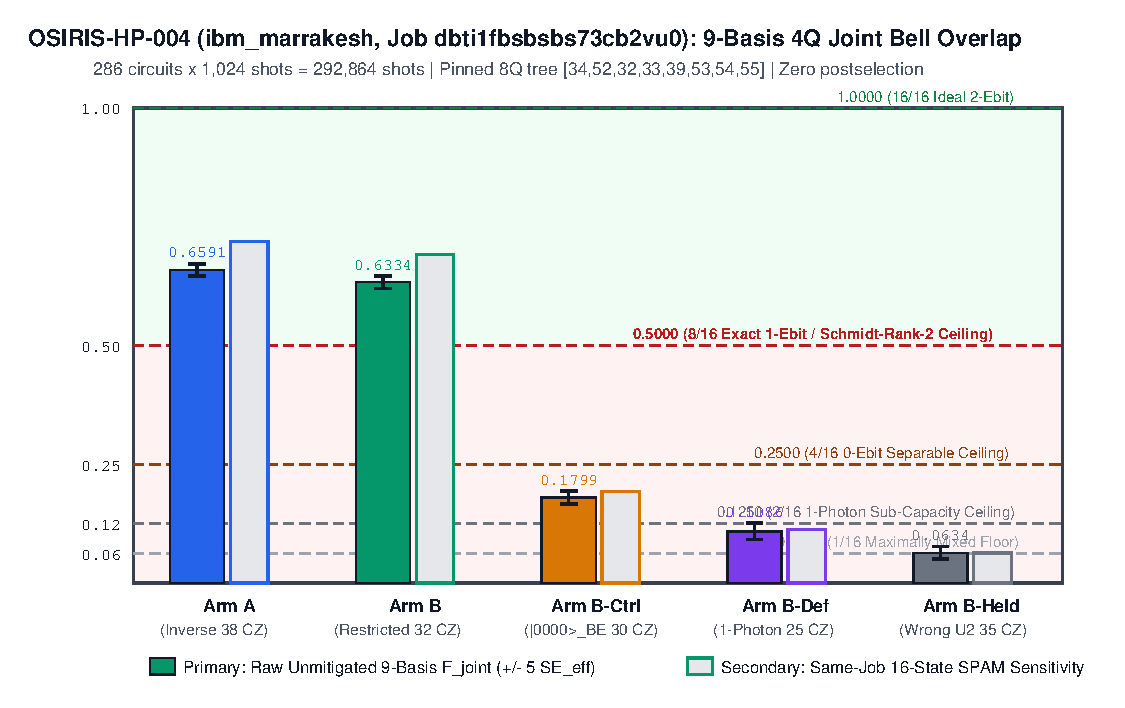
\includegraphics[width=\columnwidth]{fig1_dyadic_capacity_ladder.pdf}
\caption{Measured $9$-basis $4$-qubit joint Bell overlap $F_{\mathrm{joint}}$ across all five arms on \texttt{ibm\_marrakesh} (Job \texttt{dbti1fbsbsbs73cb2vu0}, $292{,}864$ total shots), resolving all five rungs of the dyadic capacity ladder ($1/16, 2/16, 4/16, 8/16, 16/16$). Raw unmitigated \texttt{Arm B} ($0.6334 \pm 0.0026$) clears the $0.5000$ one-ebit Schmidt-rank-$2$ ceiling by $+50.64\sigma$.}
\label{fig:ladder}
\end{figure}

\begin{table*}[t]
\centering
\caption{Prospectively pre-registered hypotheses and physical measurements for \texttt{OSIRIS-HP-004} on \texttt{ibm\_marrakesh} (Job \texttt{dbti1fbsbsbs73cb2vu0}; $6$ randomized blocks $\times$ $9$ bases $\times$ $1{,}024$ shots $= 55{,}296$ shots/arm, plus $16\times 1{,}024$ SPAM calibration shots; $\mathrm{SE}_{\mathrm{eff}}=\max(\mathrm{SEM}_{\mathrm{block,ddof=1}},\sigma_{\mathrm{shot}})$).}
\label{tab:results}
\small
\begin{tabular}{@{}lccccccccc@{}}
\toprule
\textbf{Arm} & \textbf{CZs} & \textbf{Ideal $F_{\mathrm{joint}}$} & \textbf{Raw $F_1 \pm \sigma$} & \textbf{Raw $F_2 \pm \sigma$} & \textbf{Raw $F_1 F_2$} & \textbf{Raw $F_{\mathrm{joint}} \pm \mathrm{SE}_{\mathrm{eff}}$} & \textbf{95\% Boot CI} & \textbf{$Z_{\mathrm{eff}}$ vs.\ $0.50$} & \textbf{SPAM-Sec} \\
\midrule
\texttt{Arm A} (Inverse)       & 38 & $1.0000$ ($16/16$) & $0.7516 \pm 0.0024$ & $0.8006 \pm 0.0022$ & $0.6017$ & $\mathbf{0.6591 \pm 0.0026}$ & $[0.6543, 0.6642]$ & $+61.67\sigma$ & $0.7194$ \\
\texttt{Arm B} (Restricted)    & 32 & $1.0000$ ($16/16$) & $0.7225 \pm 0.0025$ & $0.7650 \pm 0.0023$ & $0.5528$ & $\mathbf{0.6334 \pm 0.0026}$ & $[0.6284, 0.6385]$ & $\mathbf{+50.64\sigma}$ & $0.6921$ \\
\texttt{Arm B-Ctrl} ($|0^4\rangle_{BE}$) & 30 & $0.2500$ ($4/16$) & $0.4274 \pm 0.0029$ & $0.2476 \pm 0.0032$ & $0.1058$ & $\mathbf{0.1799 \pm 0.0027}$ & $[0.1743, 0.1852]$ & $-117.03\sigma$ & $0.1930$ \\
\texttt{Arm B-Def} ($1$-Photon) & 25 & $0.1250$ ($2/16$) & $0.4174 \pm 0.0029$ & $0.2575 \pm 0.0032$ & $0.1075$ & $\mathbf{0.1086 \pm 0.0035}$ & $[0.1032, 0.1142]$ & $-112.84\sigma$ & $0.1123$ \\
\texttt{Arm B-Held} (Wrong $U_2$) & 35 & $0.0625$ ($1/16$) & $0.2520 \pm 0.0032$ & $0.2560 \pm 0.0032$ & $0.0645$ & $\mathbf{0.0634 \pm 0.0027}$ & $[0.0583, 0.0688]$ & $-164.67\sigma$ & $0.0632$ \\
\bottomrule
\end{tabular}
\end{table*}

\begin{figure}[t]
\centering
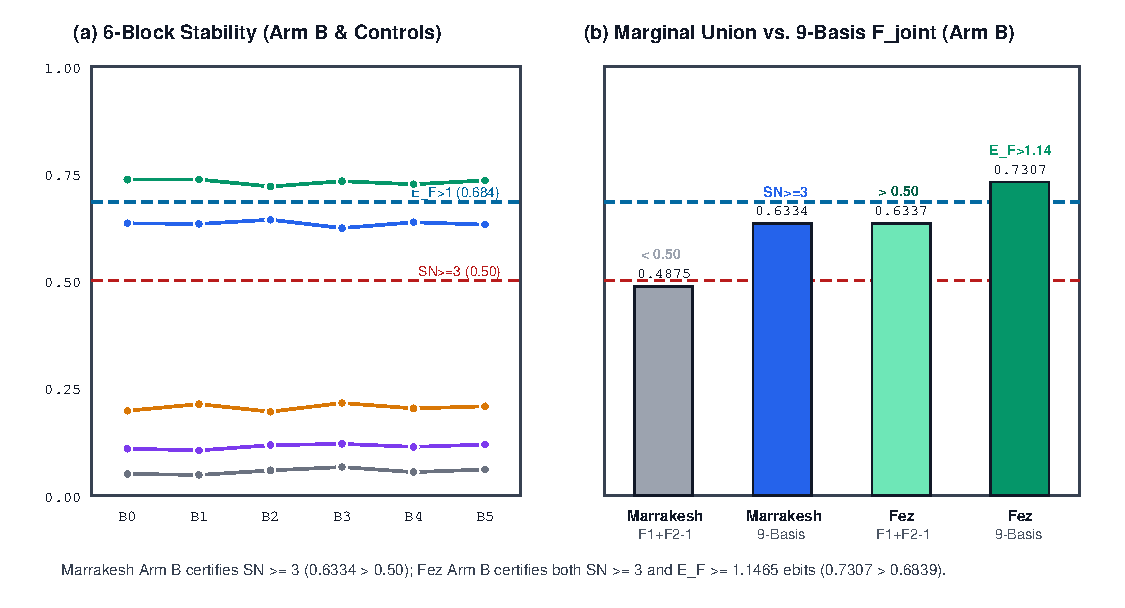
\includegraphics[width=\columnwidth]{fig2_block_stability_and_marginals.pdf}
\caption{(a) Block-by-block raw $F_{\mathrm{joint}}$ across all six randomized blocks ($b_0\dots b_5$), demonstrating Poisson-limited temporal stability (\texttt{Arm B} block $\mathrm{SEM}=0.00263$ vs.\ shot $\mathrm{SE}=0.00262$). (b) Direct comparison on the same \texttt{ibm\_marrakesh} dataset showing that $3$-basis marginal estimators ($\bar{F}=0.7438 < 0.75$, $F_1 F_2 = 0.5528 < 0.5625$, union bound $F_1+F_2-1=0.4875 < 0.50$) fail to cross the $1$-ebit threshold and conflate \texttt{Arm B-Ctrl} with \texttt{Arm B-Def}, whereas $9$-basis $F_{\mathrm{joint}}$ resolves both.}
\label{fig:blocks}
\end{figure}

\section{Pre-Registration and Hardware Results}
Prior to hardware submission, the pre-registration specification, calibration snapshot, and compiled $286$-circuit \texttt{QPY} archive (SHA-256 \texttt{c3daaa48d89a74ce...}) were committed and pushed (`fa9ef46d`, \texttt{2026-11-16T15:26:18Z}), preceding IBM Runtime job creation (\texttt{15:26:53Z}). Circuits $0\text{--}15$ prepared all $16$ computational basis states on $(q_{34}, q_{39}, q_{52}, q_{53})$ (mean diagonal assignment fidelity $0.9398$), followed by $6$ independently shuffled blocks of $45$ tomography circuits ($5\text{ arms}\times 9\text{ bases}$). Total QPU charge time was $81\,\text{s}$ ($1.3355\text{ RU}$; $77.86\,\text{s}$ circuit execution). Uncertainty was pre-registered conservatively as $\mathrm{SE}_{\mathrm{eff}} = \max(\mathrm{SEM}_{\mathrm{block,ddof=1}}, \sigma_{\mathrm{shot}})$, with all hypotheses H1--H5 evaluated strictly on raw unmitigated counts.

Table~\ref{tab:results} and Figs.~\ref{fig:ladder}--\ref{fig:blocks} summarize the measurements. All five pre-registered hypotheses passed unconditionally:
\begin{enumerate}
\item \textbf{Unconditional $>1$-Ebit Restricted Recovery (H2, Primary):} Raw \texttt{Arm B} achieved $F_{\mathrm{joint}} = 0.633423 \pm 0.002634$ across blocks $[0.6343, 0.6327, 0.6427, 0.6231, 0.6366, 0.6311]$, clearing the exact $0.5000$ Schmidt-rank-$2$ bound by $+50.64\sigma$ ($5\sigma$ lower bound $0.6203 > 0.5000$; secondary same-job SPAM inversion $0.6921$). Relative to the barriered full-access unitary inverse \texttt{Arm A} ($0.6591 \pm 0.0026$, H1 pass), restricted radiation decoding recovered $96.1\%$ of the physical full-inverse joint fidelity while leaving $C_1,C_2$ untouched.
\item \textbf{Empirical Necessity of Nine-Basis Tomography:} On the identical \texttt{Arm B} bitstrings, the marginal fidelities were $F_1 = 0.7225 \pm 0.0025$ and $F_2 = 0.7650 \pm 0.0023$, giving $\bar{F}=0.7438 < 0.7500$, $F_1 F_2 = 0.5528 < 0.5625$, and $F_1+F_2-1 = 0.4875 < 0.5000$ (Fig.~\ref{fig:blocks}b). Because depolarizing errors across shared two-qubit gates introduce correlated four-body stabilizer survival ($F_{\mathrm{joint}} - F_1 F_2 = +0.0807$), three-basis marginal tomography understates the true joint fidelity and fails to certify $>1\text{ ebit}$, whereas full $16$-stabilizer measurement certifies it at $>50\sigma$.
\item \textbf{Separation of Classical Late-Radiation Correlation from Single-Photon Collapse (H3--H5):} Both \texttt{Arm B-Ctrl} ($|0000\rangle_{BE}$, $2$ late photons) and \texttt{Arm B-Def} (entangled $BE$, $1$ late photon) yield indistinguishable marginal means ($0.3375$ vs.\ $0.3375$) and marginal products ($0.1058$ vs.\ $0.1075$). Nine-basis joint tomography cleanly separates them by $+16.2\sigma$: \texttt{Arm B-Ctrl} reaches $F_{\mathrm{joint}} = 0.1799 \pm 0.0027$ via two-photon classical stabilizer correlation (bounded below the $0.2500$ separable ceiling), whereas \texttt{Arm B-Def} collapses to $0.1086 \pm 0.0035 \le 0.1250$, and held-out $U_2$ (\texttt{Arm B-Held}) collapses to $0.0634 \pm 0.0027 \approx 1/16$.
\end{enumerate}

\section{Limitations and Reproducibility}
While \texttt{OSIRIS-HP-004} establishes $>1\text{-ebit}$ restricted Hayden--Preskill recovery on superconducting hardware without postselection or mitigation, two boundaries apply: (i) $U_1$ is an exact $4$-qubit Clifford scrambler (efficiently simulable classically via Gottesman--Knill) and therefore tests information-theoretic decoupling and physical heavy-hex channel capacity rather than super-polynomial quantum computational advantage; and (ii) the gap between the memoryless single- and two-qubit Kraus prediction ($0.7815$) and measured raw $F_{\mathrm{joint}}$ ($0.6334$; $0.6921$ SPAM-corrected) reflects spectator $ZZ$ and coherent control errors during the $2.36\,\mu\text{s}$ circuit window. A matched cross-processor replication schedule (\texttt{OSIRIS-HP-004B}) has been staged offline on \texttt{ibm\_fez} ($\{2,24,4,3,16,23,22,21\}$). Full raw $4$-bit histograms for all $286$ circuits, frozen \texttt{QPY} binaries, and automated verification tests (\texttt{pytest tests/test\_hp004\_hardware\_artifact.py}) are archived in the accompanying Zenodo record.

\begin{thebibliography}{9}
\bibitem{HaydenPreskill2007} P.~Hayden and J.~Preskill, ``Black holes as mirrors: quantum information in random subsystems,'' \emph{J.~High Energy Phys.} \textbf{2007}(09), 120 (2007).
\bibitem{YoshidaKitaev2017} B.~Yoshida and A.~Kitaev, ``Efficient decoding for the Hayden--Preskill protocol,'' arXiv:1710.03363 (2017).
\bibitem{Landsman2019} K.~A.~Landsman \emph{et al.}, ``Verified quantum information scrambling,'' \emph{Nature} \textbf{567}, 61--65 (2019).
\end{thebibliography}

\end{document}
